
\documentclass[notes=hide]{beamer}
%\documentclass[notes=only]{beamer}

\usepackage{graphicx}
\usepackage{pgfplots}
\usepackage{newcent}

\usepackage{microtype}
\usepackage{pbox}
\usepackage{multirow}
\usepackage{multicol}
\usepackage{float}
\usepackage{etex}
\usepackage{amsmath}
\usepackage[export]{adjustbox}
\usepackage{enumerate}
\usepackage{forest}
%\usepackage{tikz-qtree}
\usepackage{array}
\usepackage{graphicx} % Allows including images
\usepackage{booktabs} % Allows the use of \toprule, \midrule and \bottomrule in tables
\usepackage{amsmath,amssymb,mathtools}
\usepackage{verbatim}

\usepackage{pstricks,auto-pst-pdf}
\usepackage{tikz}
\usepackage{tikz-qtree}
 \usetikzlibrary{calc,trees,positioning,arrows,chains,shapes.geometric,%
            decorations.pathreplacing,decorations.pathmorphing,shapes,%
            matrix,shapes.symbols}
\usetikzlibrary{automata,positioning}
\usepackage{listings}
\usepackage{color}
\definecolor{mygreen}{rgb}{0,0.6,0}
\definecolor{mygray}{rgb}{0.5,0.5,0.5}
\definecolor{mymauve}{rgb}{0.58,0,0.82}
\usepackage{graphicx}
\usepackage{qtree}
\usepackage{tikz}
\usetikzlibrary{shadows,arrows,positioning}
\makeatletter
\let\@cite@ofmt\@firstofone % not \hbox
\makeatother
\setbeamertemplate{bibliography entry title}{}
\setbeamertemplate{bibliography entry location}{}
\setbeamertemplate{bibliography entry note}{}
% Define the layers to draw the diagram
\pgfdeclarelayer{background}
\pgfdeclarelayer{foreground}
\pgfsetlayers{background,main,foreground}
% Define block styles
\tikzstyle{materia}=[draw, fill=blue!20, text width=6.0em, text centered,
  minimum height=1.5em,drop shadow]
\tikzstyle{etape} = [materia, text width=8em, minimum width=10em,
  minimum height=3em, rounded corners, drop shadow]
\tikzstyle{texto} = [above, text width=6em, text centered]
\tikzstyle{linepart} = [draw, thick, color=black!50, -latex', dashed]
\tikzstyle{line} = [draw, thick, color=black!50, -latex']
\tikzstyle{ur}=[draw, text centered, minimum height=0.01em]

\usetikzlibrary{positioning}
\usetikzlibrary{fit}
\usetikzlibrary{backgrounds}
\usetikzlibrary{calc}
\usetikzlibrary{shapes}
\usetikzlibrary{mindmap}
\usetikzlibrary{decorations.text}
%\setbeameroption{hide notes}
\setbeamertemplate{note page}[plain]

% get rid of junk
\usetheme{default}
\beamertemplatenavigationsymbolsempty
\hypersetup{pdfpagemode=UseNone} % don't show bookmarks on initial view
% named colors
\definecolor{offwhite}{RGB}{249,242,215}
\definecolor{foreground}{RGB}{255,255,255}
\definecolor{background}{RGB}{24,24,24}
\definecolor{title}{RGB}{107,174,214}
\definecolor{gray}{RGB}{155,155,155}
\definecolor{subtitle}{RGB}{102,255,204}
\definecolor{hilight}{RGB}{102,255,204}
\definecolor{vhilight}{RGB}{255,111,207}
\definecolor{lolight}{RGB}{155,155,155}
\definecolor{green}{RGB}{125,250,125}
% use those colors
\setbeamercolor{titlelike}{fg=title}
\setbeamercolor{subtitle}{fg=subtitle}
\setbeamercolor{institute}{fg=gray}
%\setbeamercolor{normal text}{fg=foreground,bg=foreground}
\setbeamercolor{item}{fg=title} % color of bullets
\setbeamercolor{subitem}{fg=gray}
\setbeamercolor{itemize/enumerate subbody}{fg=gray}
\setbeamertemplate{itemize subitem}{{\textendash}}
\setbeamerfont{itemize/enumerate subbody}{size=\footnotesize}
\setbeamerfont{itemize/enumerate subitem}{size=\footnotesize}

% page number
\setbeamertemplate{footline}{%
    \raisebox{5pt}{\makebox[\paperwidth]{\hfill\makebox[20pt]{\color{gray}
          \scriptsize\insertframenumber}}}\hspace*{5pt}}

% add a bit of space at the top of the notes page
\addtobeamertemplate{note page}{\setlength{\parskip}{12pt}}

% a few macros
\newcommand{\bi}{\begin{itemize}}
\newcommand{\ei}{\end{itemize}}
\newcommand{\ig}{\includegraphics}
\newcommand{\subt}[1]{{\footnotesize \color{subtitle} {#1}}}

\author{Russell Jarvis}
\institute{
\includegraphics[scale=0.33]{logo-from-tunnel.png}}
\date{\href{http://kbroman.org}{\tt \scriptsize kbroman.org}
\\[-4pt]
\href{https://github.com/kbroman}{\tt \scriptsize github.com/kbroman}
\\[-4pt]
\href{https://twitter.com/kwbroman}{\tt \scriptsize @kwbroman}
}
\title{\large{{A Better File Format for Representing Neuron Morphology}}}   

\author{\Large{{R.~Jarvis}}}
\vfill
\date{\Large{\today}}% Date, can be changed to a custom date
\begin{document}
{
\setbeamertemplate{footline}{} % no page number here

\frame{

  \titlepage
}



% title slide

\begin{frame}
\frametitle{Introduction}
\begin{itemize}
\item The neural modelling community uses different file formats, to represent the geometry (and topology) of a neural tree.
\vfill
\item Each file format has offers different strengths and weaknesses.
\vfill
\item The different formats used leads to a lack of standards and portability in modelling work.
 
%\begin{figure}
%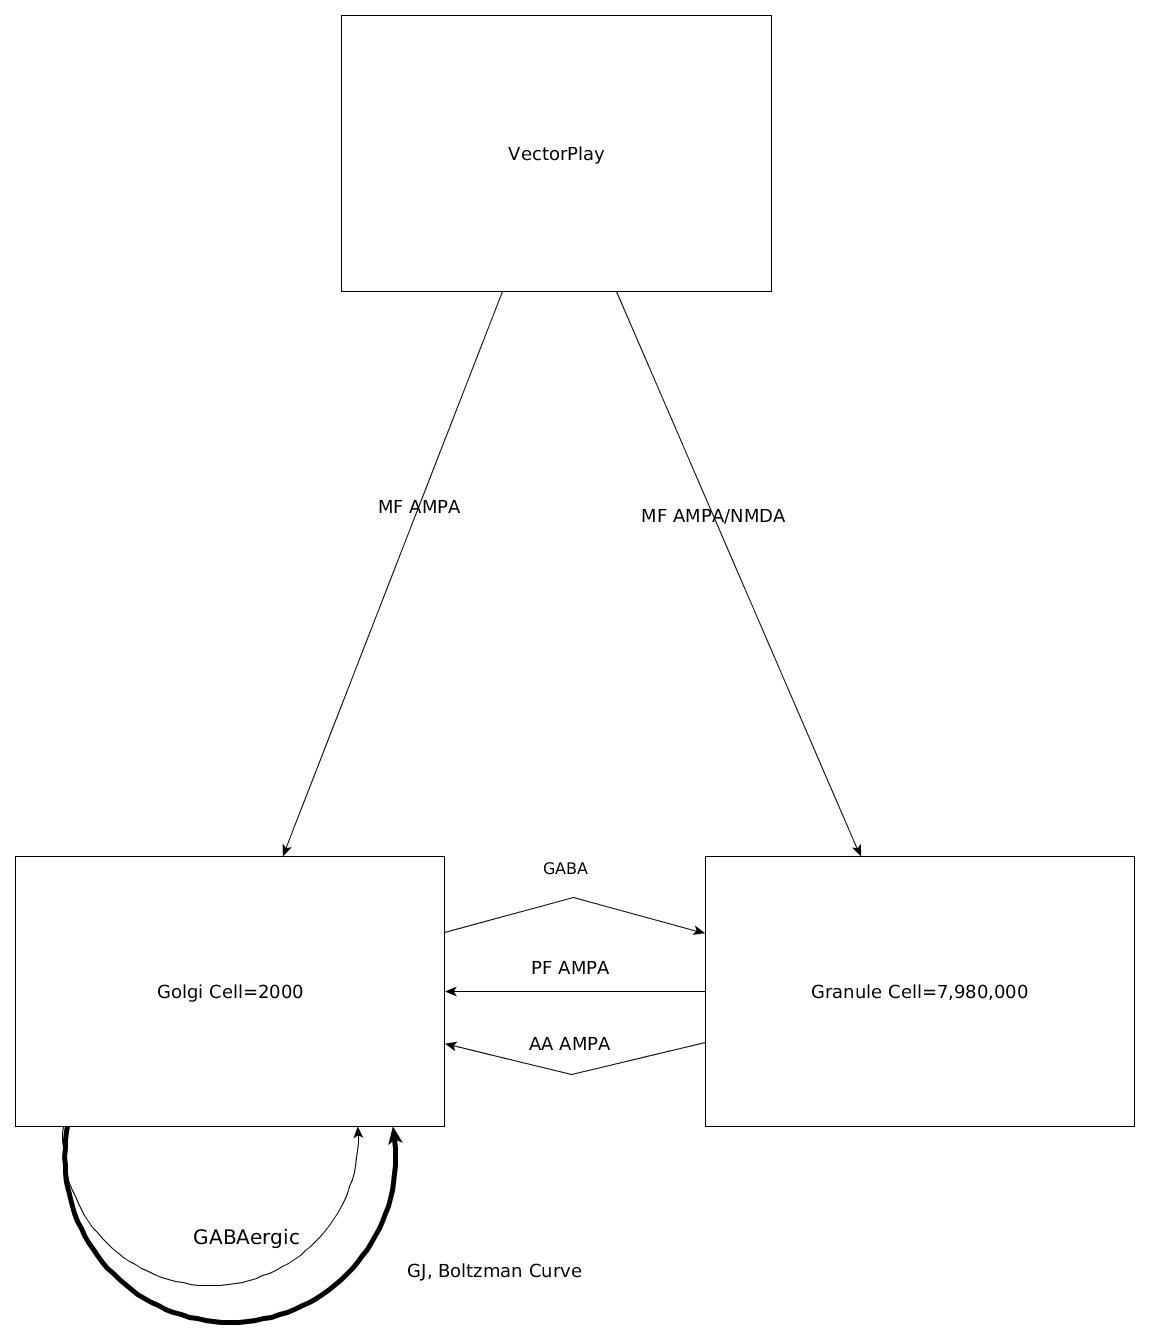
\includegraphics[scale=0.175]{Shyam_model2.jpg}
%\end{figure}
\end{itemize}
\end{frame}

\begin{frame}
\frametitle{Introduction Continued}
\begin{itemize}
\note{In the next few slides}
\item Why does the neural modelling community choose different representations of cell form?
\vfill
\note{and how this relates to the}
\item \note{I am going to} Review the strengths and weaknesses of\note{different} file formats, such that we can \note{clearly} see the limitations (barriers to universal file format). \note{that need to be overcome when creating a universal file format.} 
\end{itemize}
\end{frame}




\begin{frame}
\frametitle{SWC and Conical Frustum}
%\framesubtitle{the Most Common File Format}
\begin{itemize}
\item The traced volume of the cell is output from LM.  
\vfill
\item At each point a conical frustum is fitted to represent point of the neuron.
\vfill
\item Result is trees of connected conical frustum.
\cite{cannon1998line}.   
\note{\item GENESIS and PSICS both provide a spherical representation of the soma.}

\begin{figure}
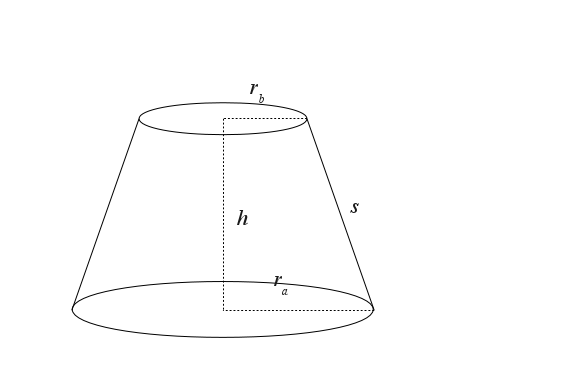
\includegraphics[scale=0.175]{conical_frustum_equation.png}
\end{figure}

\begin{figure}
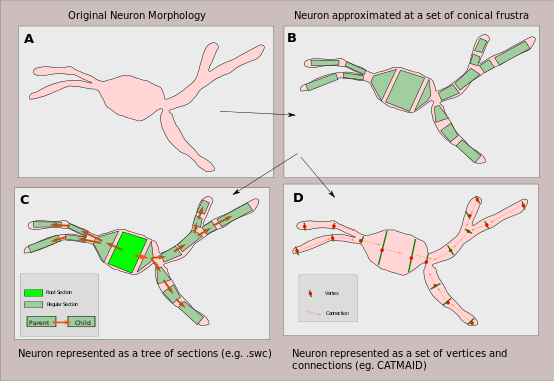
\includegraphics[scale=0.3]{new_morphology_original.jpg}
\end{figure}
\cite{rahim2012curve}
\end{itemize}


\end{frame}


\begin{frame}
\frametitle{SWC}
\begin{figure}
\begin{itemize}
\item The \textbf{C} and \textbf{ID} columns can be regarded as a sparse form of an adjacency matrix.
\end{itemize}
\vfill
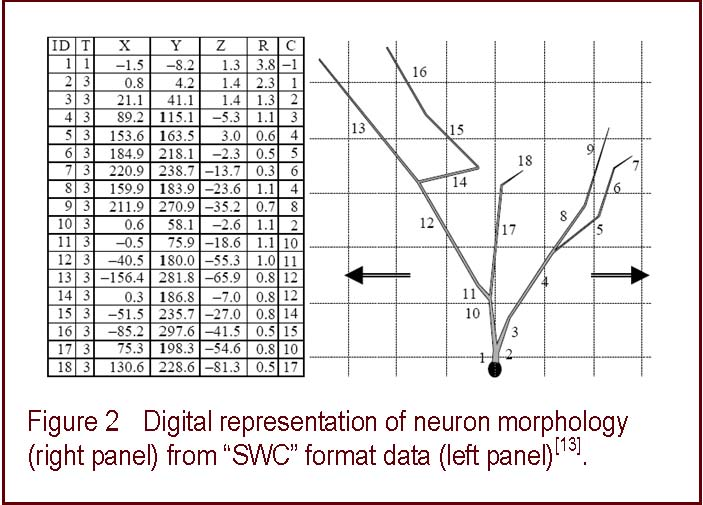
\includegraphics[scale=1.05]{NeuralRegenRes_2012_7_21_1637_128269_2.jpg}
\end{figure}
\cite{rahim2012curve}
\end{frame}


\begin{frame}
\begin{itemize}
\frametitle{Why is SWC so popular?}

\item Good compromise between representing geometric variability and achieving computational tractability.
\vfill
\item This system of spatial discretization eases indexing and recording from ROI.
\vfill
%\begin{itemize}  
%	\item a natural consequence of the SWC representation. 
%\end{itemize}
%\vfill
\item Also eases splitting the cell trees over multiple CPUs
\cite{eichner2009neural}.
\vfill
\end{itemize}
\end{frame}
\begin{frame}
\frametitle{Why SWC is not the desired standard?}

\begin{itemize}
\item The frustum is limited in how well it can represent variations in surface, and such variations are important determinants of neuron excitability.
\vfill
\item Not suited to representing spines or myline \cite{slezak2014brain}.
\vfill
%\item Minimum number of standard membrane domains.
%\vfill
\item Within neuromorpho no minimum quality of reconstruction, or header information \cite{slezak2014brain}. 
%\vfill
%\item SWC is not expressed in XML, and it cannot easily sit inside a bigger data container that geometrically describes a forest.
\end{itemize}
\end{frame}


\begin{frame}
\frametitle{MATLAB toolbox Trees}
%\framesubtitle{A trees connectivity can be Represented in data structure}
\begin{itemize}
\item Trees is based on the idea that neuron connectivity can be represented by two or more binary trees (graphs). 
\vfill

%Therefore file formats must prevent the specification of ternary trees.\
\note{The matrix representation of connectivity can be efficiently stored as a string or gene tree, however the geometric information cannot be compressed any further.
}
%\vfill
%\item Row elements represent parents, column elements represent children.
\end{itemize}
\begin{figure}
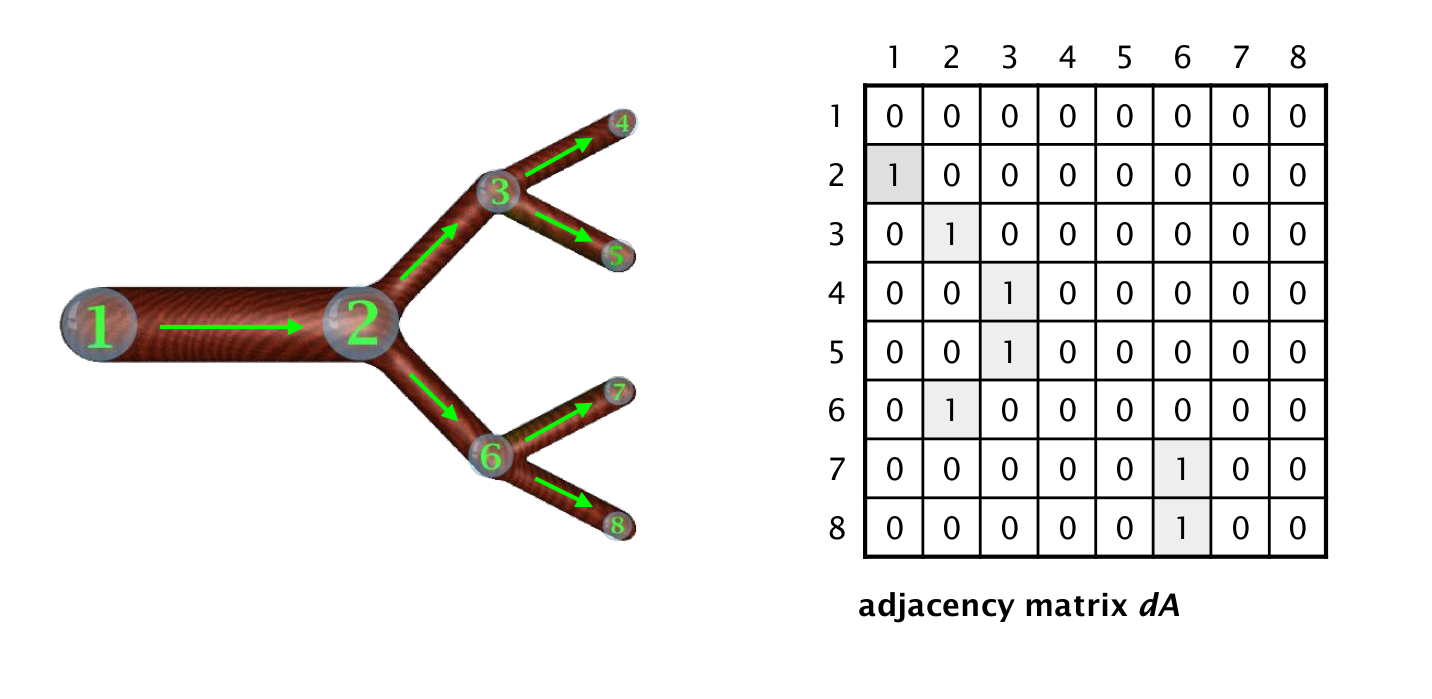
\includegraphics[scale=0.2]{topology_tree2.png} 
\end{figure}
\vfill
\cite{cuntz2011trees}
%\cite{mcdougal2013reaction}
\end{frame}




\begin{frame}
\frametitle{MATLAB Trees: Benefits and Drawbacks} 

\begin{itemize}
\item \textbf{Benefits}
\begin{itemize}
\item Matrix representation of connectivity convenient for morphometric analysis comparison and editing tree morphology.
\end{itemize}

\vfill
\item \textbf{Why is it not the standard?}
\vfill
\begin{itemize}

\item The type of geometry representation is not a mesh.
\vfill
%\item As with SWC the symmetrical frustum does not represent surface and volume well enough at sites where reaction diffusion is important.
%\vfill
%\item As with SWC does not represent spines or vesicle release sites.
%\vfill
\item Neither Trees or SWC represent time varying structural changes.
\vfill
\item Although can output .swc, .mtr extension saves a MATLAB workspace.
\end{itemize}

\end{itemize}
\end{frame}

\begin{frame}
\frametitle{MorphML}

\tiny
\def\CUP{{\bf cup}}
\def\Nspec{N$_{\mbox{\sc spec}}$}
\Tree [.Morphml
 [.Cells
 [.Cell
   [.segments
     [ 0th-segment-coordinates ] [ .... ][ Nth-segment-coordinates ]
   ]
   [.cables
     [ 0th-cable ] [ .... ][ Nth-cable ]
   ]
 ].Cell % repeated label
]
]
\end{frame}
%\begin{frame}
%\frametitle{MorphML: strengths and weaknesses}
%\small
%\begin{itemize}
%\item \textbf{Why Do they use it?}
%\vfill
%\item Since its XML can be easily nested in a bigger data container.
%\vfill
%\item \textbf{Why is it not a standard?}
%\vfill
%\item Merely an XML version of SWC so it inherits all of SWCs limitations.
%\vfill
%\item Cable group specified twice. Redundant.
%%\item Just like SWC only describes cylinders not mesh surfaces.
%%\item terminology: A section is a cylinder composed of smaller fixed radius elements called segments. 
%%\item in this context, cable also refers to a cylinder composed of smaller fixed radius elements.
%\end{itemize}
%
%\end{frame}


\begin{frame}
\frametitle{Mesh Can Better Represent Variation in Surface}
%\framesubtitle{}
%\vfill
\begin{itemize}

\item Varying geometry of surface effects electrotonic compactness
\begin{itemize}
\item and firing patter of the neuron \cite{mainen1996influence}.
\end{itemize}
\item Alters passive resistance to current following synaptic input.  
\vfill  
\item Surface geometry important to Reaction Diffusion.
\end{itemize}
\hfill
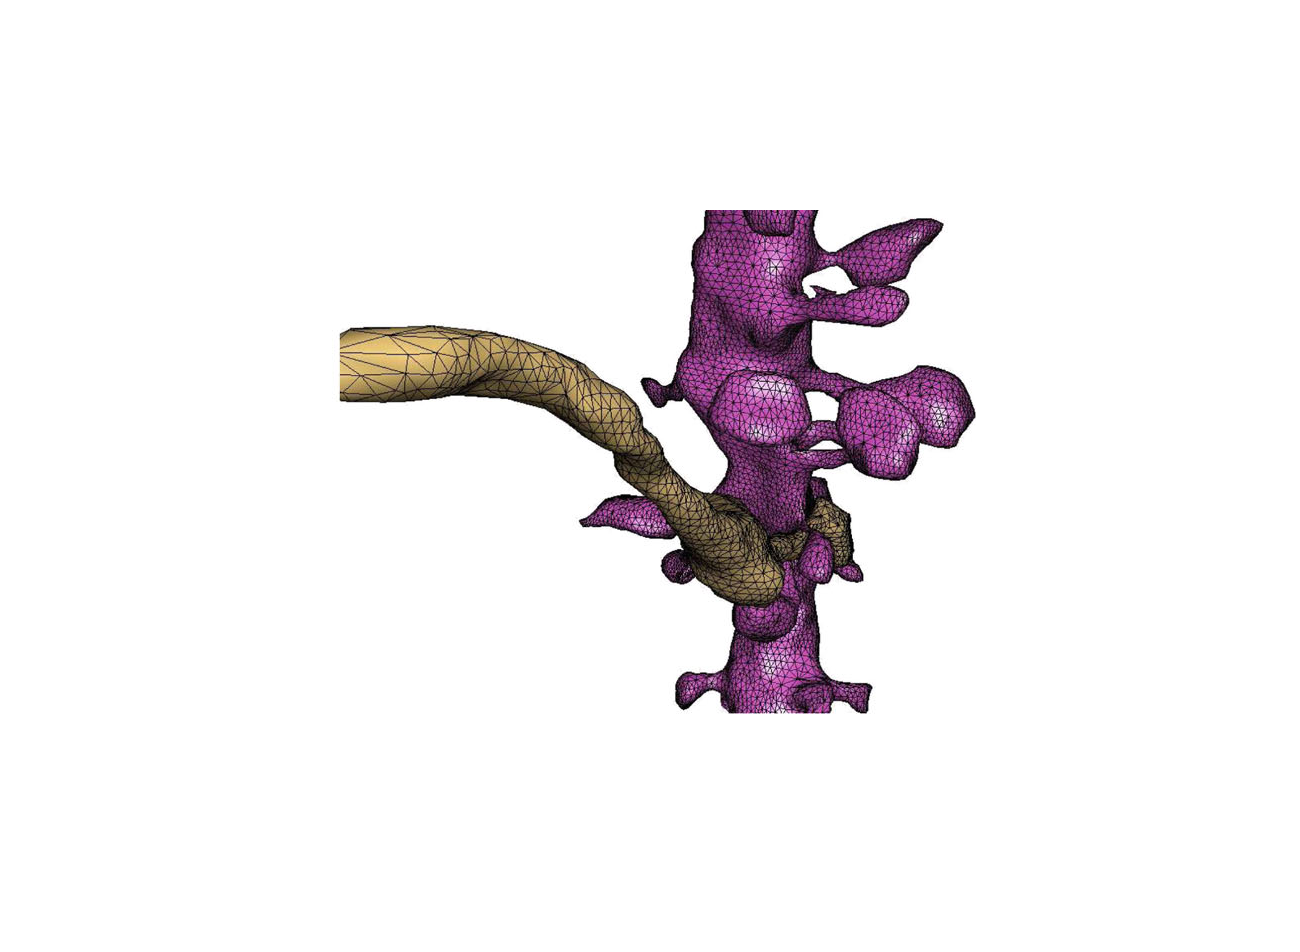
\includegraphics[scale=0.15]{spines2.png} \cite{edwards2014volrovern}


\end{frame}

%\begin{frame}
%\begin{figure}

%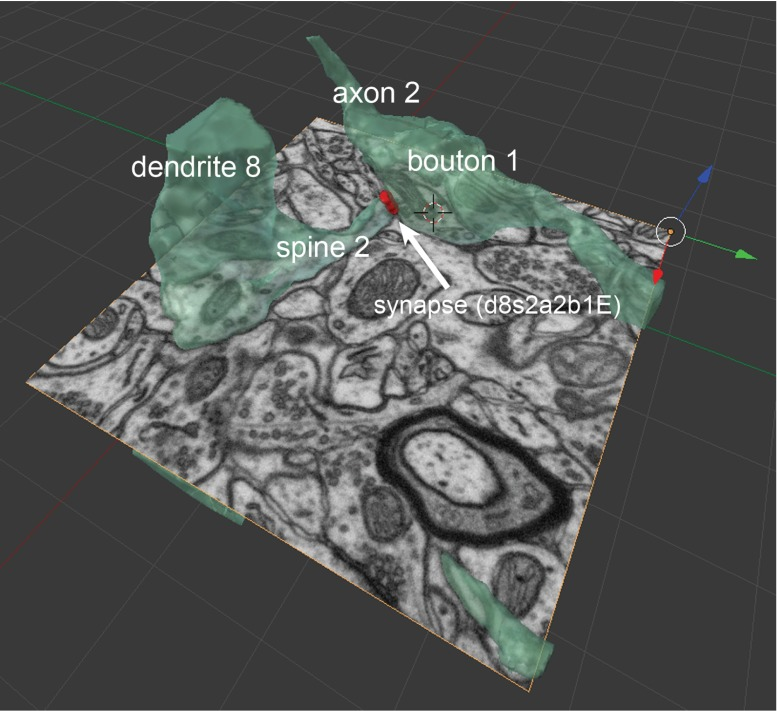
\includegraphics[scale=2.25]{spine.jpg}
%\end{figure}
%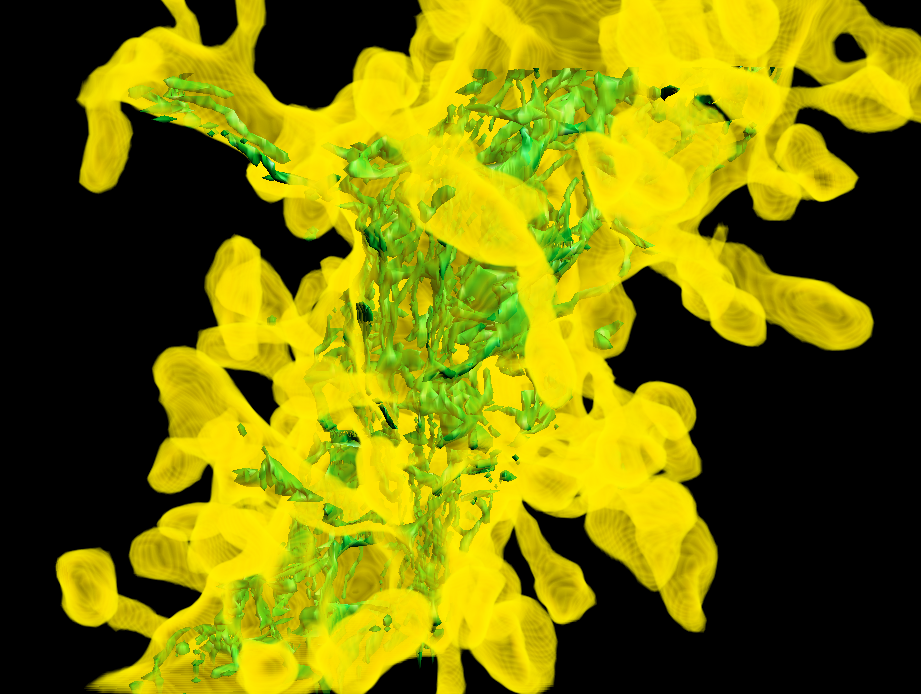
\includegraphics[scale=2.25]{ER_inside_spines.png}

%\end{frame}

\begin{frame}[fragile]
\frametitle{STereoLithography (STL) and Polygon surface}
%where name is an optional string (though if name is omitted there must still be a space after solid). The file continues with any number of triangles, each represented as follows:
%\begin{itemize}
%\item Describes a polygon triangle in a volume three points at a time.
%\item The facet normal is redundant as it can be inferred from the coordinates of the three vertices.
%\end{itemize}
\hfill 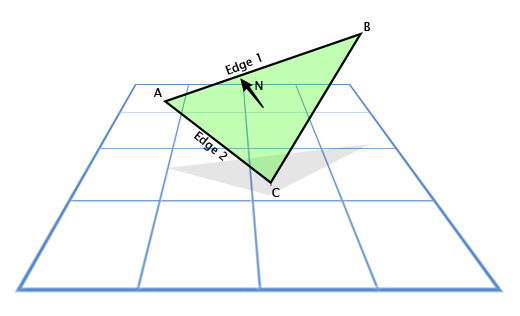
\includegraphics[scale=0.3]{facet_normal.jpg}\hfill\hfill
%\rotatebox[origin=c]{90}{anti-clockwise}

\begin{lstlisting}
solid name
	facet normal ni nj nk
		outer loop
		    vertex v1x v1y v1z
		    vertex v2x v2y v2z
		    vertex v3x v3y v3z
		endloop
	endfacet
endsolid name
\end{lstlisting}
%\right\downarrow
%The 3D printing community is also outgrowing this file format, for different reasons.
%\]'\]'

\end{frame}

\begin{frame}
\frametitle{Tetrahedron Mesh Formats}
\begin{itemize}
\item A tetrahedron is a pyramid volume enclosed by 4 vertices and 6 edges.
\end{itemize}
\begin{figure}
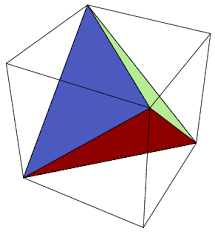
\includegraphics[scale=0.55]{tetra.png}

%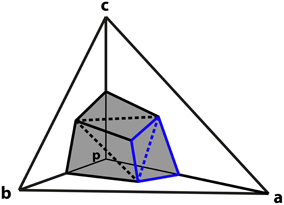
\includegraphics[scale=0.55]{fncom-07-00129-g001.jpg}
\end{figure}
\end{frame}



\begin{frame}[fragile]
\frametitle{Abaqus (.inp)}
\begin{verbatim}
Data line 
*NODE
*NODE
101, 0., 0., 0.
102, 1., 0., 0.
103, 2., 0., 0.

Connectivity
*ELEMENT, TYPE=T2D2, ELSET=
FRAME
11, 101, 102
12, 102, 103 
13, 101, 104 
14, 102, 104 

\end{verbatim}
\end{frame}

\begin{frame}
\frametitle{Abaqus and STL Why Are they Used?}
\begin{itemize}

\item Surfaces are a good model for reaction diffusion.
\vfill
\item In the case of Abaqus. Dendrite Spine Endoplasmic Reticulum can be represented, which is important for reaction diffusion.
\vfill
\item The membrane potential can be evaluated on and between vertices using STEPS.

\end{itemize}
\end{frame}

\begin{frame}
\frametitle{So Why doesn't everyone Use Abaqus and STL?}
\begin{itemize}

\vfill
\item Less computationally tractable esp. for network scale simulations.
\vfill
\item Discretization not simple, vertices not clearly in or out of conical ROI.
\vfill
\item Current injection into membrane requires defining direction of current flow from outside to inside the cell (unlike NEURON/GENESIS).
\vfill
\item Splitting trees across CPUs not simple since mesh vertices much more interconnected than conical frustum.
%\vfill 
%\item software that edits on Abaqus files not Open Source.
%\vfill
%\item Unlabelled trees and membrane domains.

\end{itemize}
\end{frame}


\begin{frame}
\frametitle{Multisplit Trees}
\begin{itemize}
\item To make dynamic simulations computationally tractable. Neuron trees can be split up and simulated on different CPUS.
\item When solving the cable equation dependence between nodes is important.
\end{itemize}
\vfill
\begin{figure}
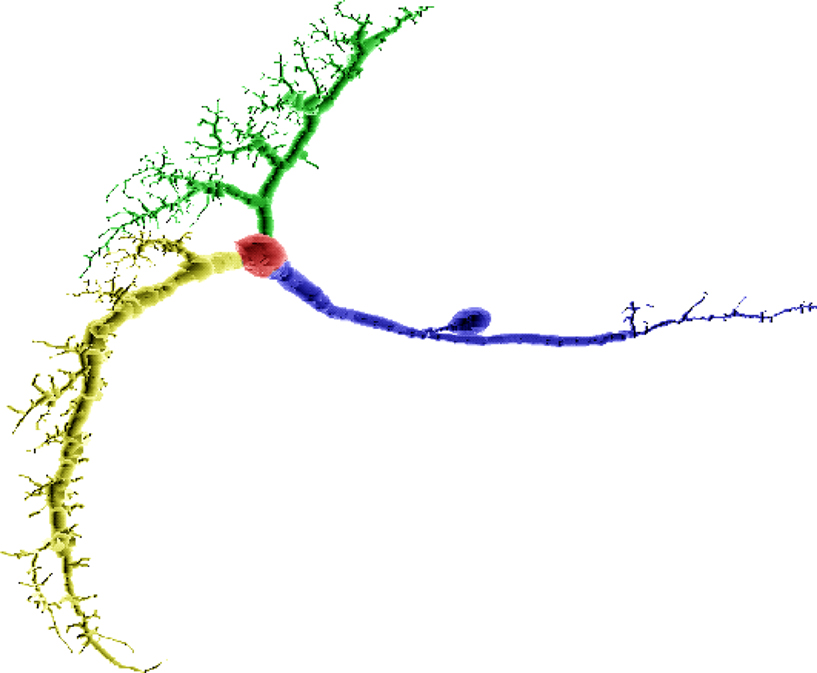
\includegraphics[scale=0.85]{fninf-03-021-g009.jpg}
\end{figure}
\cite{eichner2009neural}
\end{frame}

\begin{frame}
\frametitle{Synthetic Morphologies}
\begin{itemize}
\item NeuroMAC output provides pre-synaptic and post-synaptic coordinates, in addition to cell id's. 
\vfill
\item An adj. matrix is lacking, there is no standard for multidimensional connectivity information.
\vfill
\item Given NeuroMAC, NETMORPH, CX3D and Neugen the future should include dynamic sim. in \note{forests} of time-varying neuron structure.
\vfill
\begin{itemize}
\item \cite{torben2014context} 
\cite{bito2010chemical}
\cite{eberhard2006neugen}
\end{itemize}
\end{itemize}
\end{frame}

\begin{frame}

\frametitle{Optomize Tradeoff: Computational tractability vs Biophysical Accuracy.}
\begin{itemize}
\begin{itemize}
\item Optomize representation by using tetrahedra surface mesh at dendrite spines conical frustum everywhere else.
\item \cite{hepburn2013efficient} \cite{grein20141d} \cite{bito2010chemical}%\item Use normal vector to describe how mesh is orientated relative to a position on the frustum.
%\vfill
%\item Automatically resolving overlaps difficult. 

\vfill
\end{itemize}

\begin{figure}
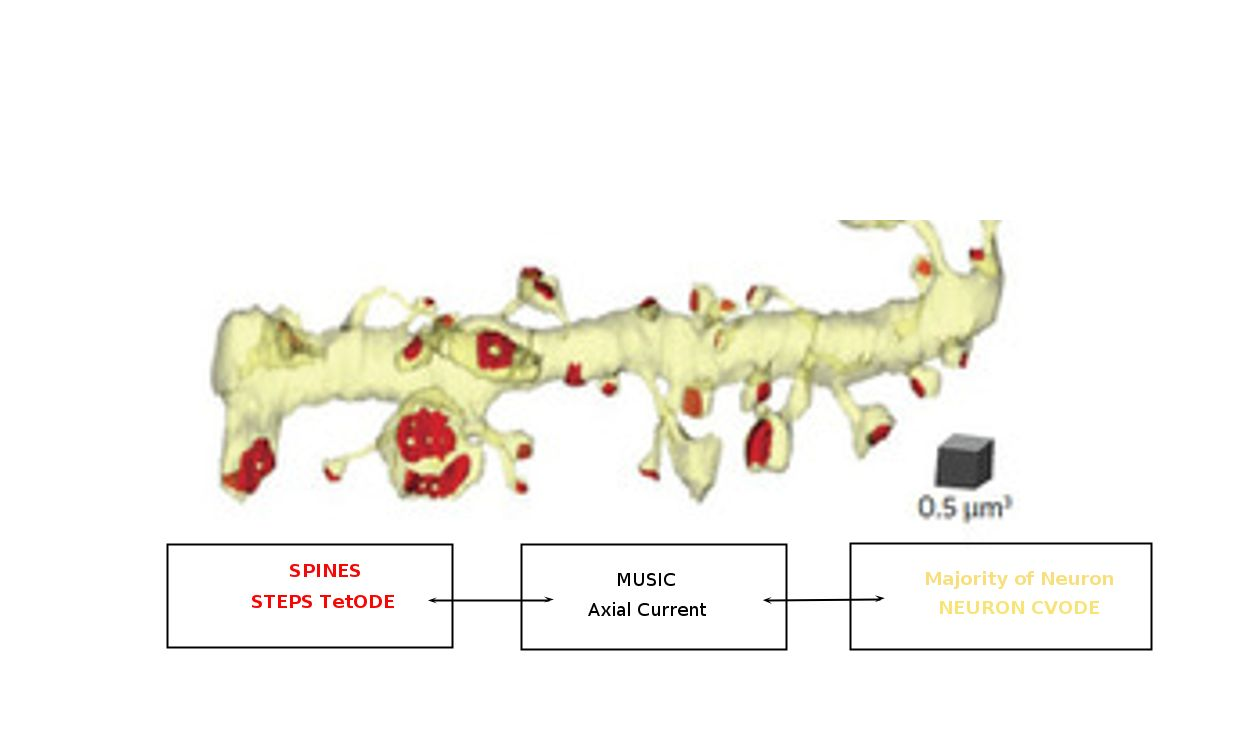
\includegraphics[scale=0.27525]{multisimulatorinterface2.jpg}
\end{figure}
\end{itemize}
\vfill
\vfill

\end{frame}

\begin{frame}
\frametitle{Use Case: New morphology file format}

%Use Case: Digitally represent the spatial information of a cell.
\begin{itemize}
\item Primary Actors: Neuroscientists %: (dynamic neural modellers and morphometric analysis).
\vfill
\item Stakeholders: Neuroscientists investigating any or all of: 
\begin{itemize}
\item Statistics of the tree structure of neurons
\item Electrophysiology in neurons and networks
\item Connectivity in forests of neurons.
\end{itemize}
\vfill
\item Scope: Representing the time varying or static geometry and topology of a single neuron, or a connected forest of neurons.
\vfill
\item Level: Sub function -
\end{itemize}
\end{frame}

\begin{frame}
\frametitle{Use Case: continued}
\begin{itemize}
\vfill 
\item Triggers:
Actor has completed nano-meter resolution neural imaging, image stack is available for dynamic or structural modelling. 
\vfill
\item Preconditions:
Available polygon mesh nodes and vertices of manifolds.
\vfill
\item Success Guarantees:
\begin{itemize}
\item More accurate results than achieved via 1D exclusive use of the 1D cable equation. 
\item The solver exploit FEM simulation at the area of the spine.
\item simulation executes faster
\item Lesser RAM/CPU burden than with a full FEM simulation.
\item Dynamic simulations with time varying structural plasticity are not be made impossible by the file format.
\end{itemize}
\end{itemize}
\end{frame}


\begin{frame}
\frametitle{Recommendations for New File Format}
\begin{itemize}
\item Should be HDF5 \&\& XML.
\vfill
\item XML allows nesting of meta data at any level of resolution.
\vfill 
\item Also XML documents facilitate the nesting of cell geometries in a forest. 
\vfill
\item Should be a data container for two types representation (mesh and frustum).

\vfill
\item Needs to load balance friendly.
\vfill
\item Should not make it harder to make a time series extension. 
\end{itemize}
\end{frame}




%\begin{frame}
%\frametitle{Brain Storm of File Format-Concept}


%\def\CUP{{\bf cup}}
%\def\Nspec{N$_{\mbox{\sc spec}}$}
%\resizebox{\linewidth}{!}{%
%\Tree [.NineML
% [.Population 
% [.Cell 
%    [.adjacency-matrix
%     [ column-parents ][ row-children ]
%    ]
%   [.frustum-end
%     [ frustum-end-coordinates ][ frustum-end-radius ]
%   ]
%   [.domains
%     [.segment-domain ].segment-domain [ volume-domain ]
%   ]
%   [.tetrahedral-matrices vertices-coords vertices-connectivity %].tetrahedral-matrices
%   [.time-varying-dim ].time-varying-dim
% ].Cell % repeated label
%]
%]
%}
%[ post-synaptic-entities coordinates ].Network
   

%\end{frame}



\begin{frame}
\frametitle{Conclusion}
\begin{itemize}
\item In this presentation, I have: 
\vfill
\item Described the limitations of existing morphology file format.
\vfill
\item Described the trade off between computational tractability and biophysical/geometric accuracy.
\vfill
\item Proposed possible XML tree structures of a NINEML extension universal morphology file format.
\end{itemize}
\end{frame}


\begin{frame}[allowframebreaks]
\nocite{edwards2014volrovern}
\nocite{rall1964theoretical}

\bibliographystyle{apalike}
\bibliography{new}
\end{frame}

\begin{frame}
\frametitle{Are there any Questions?}
\center
\large
Thank-you For your Attention

\end{frame}
\end{document}
